
\section{Multistep interpolants for zero-cost defect control for a Runge Kutta method}
\label{section:equipping_rk4_with_HBs}
In this section we will consider a multistep interpolant approach, built on the classical $4^{th}$ order Runge Kutta method (RK4), that allows for defect control. We will augment the discrete Runge-Kutta solution with interpolants of $4^{th}$, $6^{th}$ and $8^{th}$ orders respectively and explain the challenges and the efficiency and accuracy of each interpolant. 

We first note that Runge-Kutta methods are very convenient in that they are one step methods. At any point, when taking the next step, the method does not have to take into consideration the size of the previous steps and this is convenient as the solver can choose the size of the next step in the most optimal way based only on how the error estimate compares with the tolerance for the current step. 

The first interpolant that we discuss is a single step interpolant. It is the classical Hermite cubic of order 4. We will show how this interpolant can be used to perform defect control and discuss the limitations of this interpolant. 

We then show how a Hermite-Birkhoff interpolant of $6^{th}$ order can address the issues that we identified for the $4^{th}$ order interpolant. We will give an overview of how a $6^{th}$ order interpolant is derived and show the results of applying defect control using this interpolant to solve the three test problems. 

We will then use a similar approach to derive an $8^{th}$ order Hermite-Birkhoff interpolant and show why the approach used for the $6^{th}$ order interpolant needs to be modified for the $8^{th}$ order. We then discuss another approach to derive an $8^{th}$ order interpolant that addresses the issue with the previous one and show the results of using this $8^{th}$ order interpolant as the basis for computing defect controlled numerical solutions of the three test problems.


\subsection{The Classical $4^{th}$ order RK method with a $4^{th}$ order Hermite Cubic Interpolant}
The Hermite cubic spline is a very widely used interpolant. The basic idea is that we can use the derivative values and not just the solution values to get more data to fit an interpolant. Given points $(t_i, y_i)$ and $(t_{i + 1}, y_{i + 1})$ with derivatives $f_i$ and $f_{i + 1}$ (here $f_i = f(t_i, y_i)$ and $f_{i+1}=f(t_{i+1}, y_{i+1})$), respectively, the interpolant across the step $[t_i, t_{i + 1}]$ of size $h_i$ is defined as:

\begin{equation}
\label{eqn:HB4}
u(t_i + \theta h) = h_{00}(\theta)y_i +  h_ih_{10}(\theta)f_i + h_{01}(\theta)y_{i + 1} + h_ih_{11}(\theta)f_{i + 1}, 
\end{equation}
and its derivative is:
\begin{equation}
u'(t_i + \theta h) = h_{00}'(\theta)y_i/h_i +  h_{10}'(\theta)f_i + h_{01}'(\theta)y_{i + 1}/h_i + h_{11}'(\theta)f_{i + 1}. 
\end{equation}

The quantity $\theta$ is:
\begin{equation}
\label{eqn:HB4_theta}
\theta = (t - t_i) / h_i.
\end{equation}

The functions $h_{00}(\theta)$, $h_{01}(\theta)$, $h_{10}(\theta)$ and $h_{11}(\theta)$ are each cubics defined such that $u(t_i)= y_i$, $u'(t_i) = f_i$, $u(t_{i+1}) = y_{i + 1}$ and $u'(t_{i + 1}) = f_{i + 1}$. When $\theta$ is 0, $t_i + \theta h_i$ is $t_i$ and thus only $h_{00}(0)$ should be 1 and all the others cubic should evaluate to 0. Also only $h_{10}'(0)$ should be 1 and the derivatives of all the other cubics should evaluate to 0. When $\theta$ is 1, $t_i + \theta h_i$ is $t_{i + 1}$ and thus only $h_{01}(1)$ should be 1 and all the other cubics should evaluate to 0. Also only $h_{11}'(1)$ should be 1 and the derivatives of all the other cubics should be 0.

We will assume that each of the cubics has the form $a\theta^3 + b\theta^2 + c\theta + d$, where $a, b, c$ and $d$ are coefficients to be determined, and note that for each cubic we know its value for $\theta$ at 0 and 1 and the values of its derivatives for $\theta$ at 0 and 1. We thus have 4 equations for each cubic. Thus we can solve the system for each cubic to get the values of a, b, c and d for each cubic.

We now note that from equations $\ref{eqn:HB4}$ and $\ref{eqn:HB4_theta}$, we can evaluate both the interpolant and its derivative for any $\theta$ in $[t_i, t_{i + 1}]$ and therefore we can form $\delta(t + \theta h_i) = u'(t_i + \theta h_i) - f(t_i + \theta h_i, u(t_i + \theta h_i))$ which can be used to sample the defect for any $\theta$.

We will show below experimentally that the maximum defect occurs consistently approximately either at $x_i + 0.2h_i$ or at $x_i + 0.8h_i$ so that we just need to sample the defect twice in order to obtain an estimate of the maximum defect on the step.

We now note that the interpolant comes at no additional cost. We only need $(x_i, y_i, f_i)$ and $(x_{i + 1}, y_{i + 1}, f_{i + 1})$ to be stored as the discrete solution approximation are computed by the RK method. No additional stages or function evaluations are required for the construction of the interpolant itself. 

For the remainder of this chapter, we will refer to the Hermite cubic interpolant as `HB4'.

\paragraph{Problem 1 results}
Figures $\ref{fig:rk4_with_hb4_p1_global_defect}$, $\ref{fig:rk4_with_hb4_p1_global_error}$ and $\ref{fig:rk4_with_hb4_p1_scaled_defects}$ shows the results of using RK4 with HB4 on Problem 1. We note that an absolute tolerance of $10^{-6}$ is applied on the maximum defect estimate within the step and this can be observed to occur at $0.2h$ and $0.8h$ for a step of size h. See Figure $\ref{fig:rk4_with_hb4_p1_scaled_defects}$, to see the scaled defect reaching a maximum near these points. (The figure shows the shape of the defect for each of the steps that were taken to solve Problem 1 using RK4 with HB4. All the defects were scaled vertically to be in the range [0, 1] and scaled horizontally so that they map onto [0, 1]. We see that over all steps and problems, the defect has two clear peaks at $0.2h$ and $0.8h$.) We note that we are able to successfully control the defect of the continuous numerical solution using this approach; see Figure $\ref{fig:rk4_with_hb4_p1_global_defect}$. To obtain these results, we sampled the defect at many points within each step.

\begin{figure}[H]
\centering
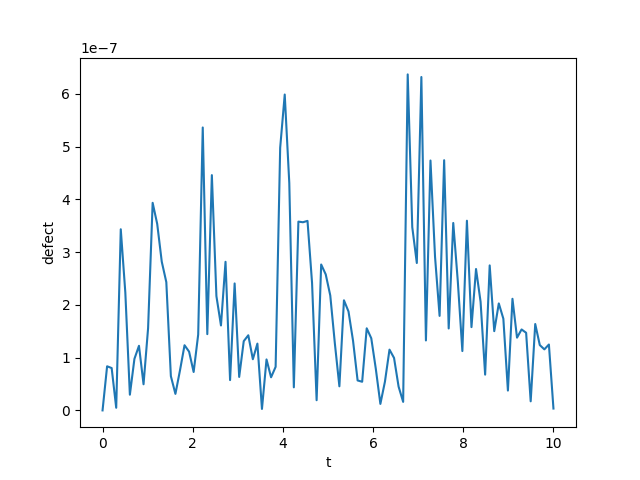
\includegraphics[width=0.7\linewidth]{./figures/rk4_with_hb4_p1_global_defect}
\caption{Defect across the entire domain for RK4 with HB4 on problem 1 at an absolute tolerance of $10^{-6}$.}
\label{fig:rk4_with_hb4_p1_global_defect}
\end{figure}

\begin{figure}[H]
\centering
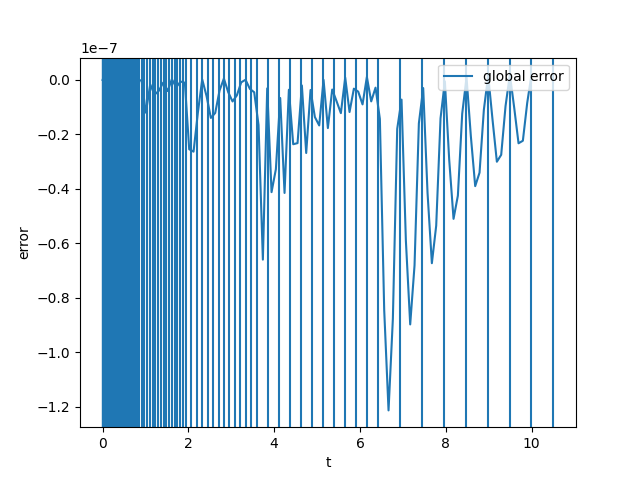
\includegraphics[width=0.7\linewidth]{./figures/rk4_with_hb4_p1_global_error}
\caption{Global Error for RK4 with HB4 on problem 1 at an absolute tolerance of $10^{-6}$.}
\label{fig:rk4_with_hb4_p1_global_error}
\end{figure}

\begin{figure}[H]
\centering
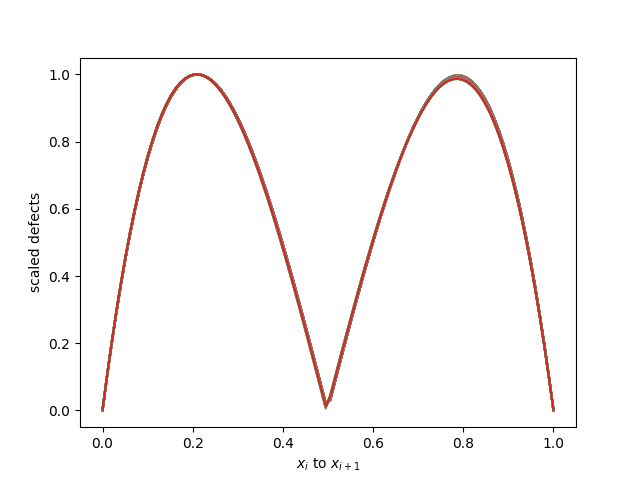
\includegraphics[width=0.7\linewidth]{./figures/rk4_with_hb4_p1_scaled_defects}
\caption{Scaled defects over all steps for RK4 with HB4 on problem 1 at an absolute tolerance of $10^{-6}$ mapped onto $[0, 1]$. The defect has the same shape on every step.}
\label{fig:rk4_with_hb4_p1_scaled_defects}
\end{figure}

\paragraph{Problem 2 results}
Figures $\ref{fig:rk4_with_hb4_p2_global_defect}$, $\ref{fig:rk4_with_hb4_p2_global_error}$ and $\ref{fig:rk4_with_hb4_p2_scaled_defects}$ shows the results of using RK4 with HB4 on Problem 2. We note that an absolute tolerance of $10^{-6}$ is applied on the maximum defect estimate within the step and this can be observed to occur at $0.2h$ and $0.8h$ for a step of size, h. See Figure $\ref{fig:rk4_with_hb4_p2_scaled_defects}$, to see the scaled defect reaching a maximum near these points. We note that we are able to successfully control the defect of the continuous numerical solution using this approach; see Figure $\ref{fig:rk4_with_hb4_p2_global_defect}$. For Problem 2, the defect is noisy on small steps and we do not get two clean peaks. However, we note that we quite consistently get the maximum defects at $0.2h$ and $0.8h$ and thus we only require two defect samplings.

\begin{figure}[H]
\centering
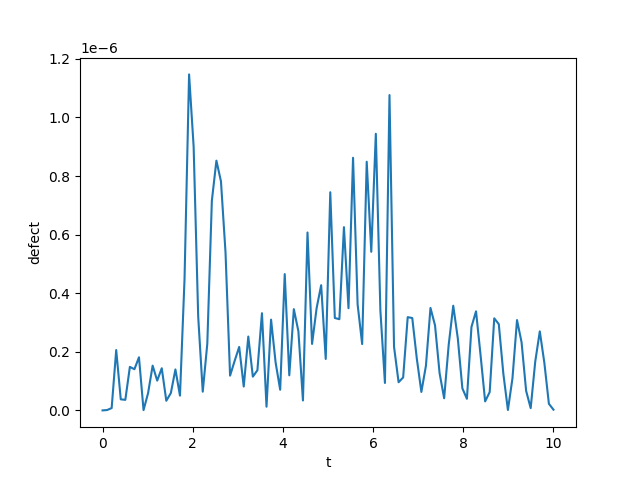
\includegraphics[width=0.7\linewidth]{./figures/rk4_with_hb4_p2_global_defect}
\caption{Defect across the entire domain for RK4 with HB4 on problem 2 at an absolute tolerance of $10^{-6}$.}
\label{fig:rk4_with_hb4_p2_global_defect}
\end{figure}

\begin{figure}[H]
\centering
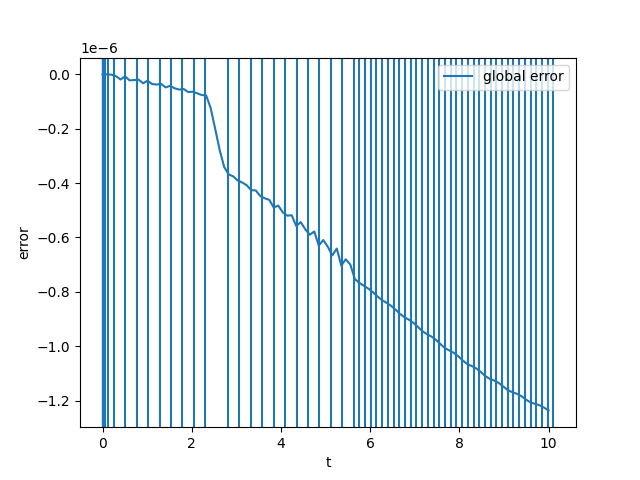
\includegraphics[width=0.7\linewidth]{./figures/rk4_with_hb4_p2_global_error}
\caption{Global Error for RK4 with HB4 on problem 2 at an absolute tolerance of $10^{-6}$. There is more variation in the shape of the defect for this problem but the maximum defect occurs near either $0.2h$ or $0.8h$.}
\label{fig:rk4_with_hb4_p2_global_error}
\end{figure}

\begin{figure}[H]
\centering
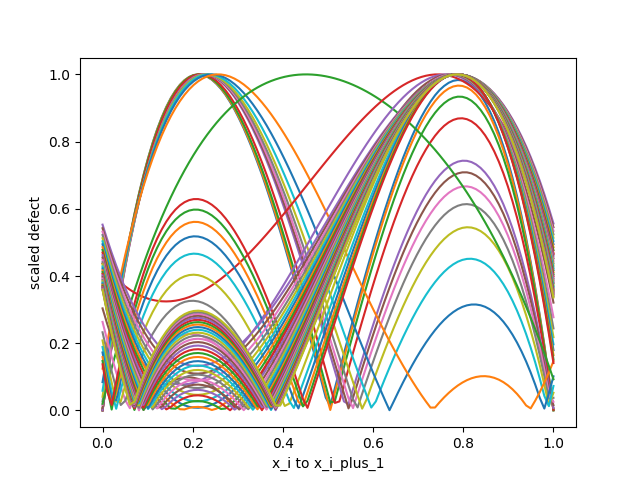
\includegraphics[width=0.7\linewidth]{./figures/rk4_with_hb4_p2_scaled_defects}
\caption{Scaled defects over all steps taken for RK4 with HB4 on problem 2 at an absolute tolerance of $10^{-6}$ mapped onto $[0, 1]$. There is more variation in the shape of the defect for this problem but the maximum defect occurs near either $0.2h$ or $0.8h$. }
\label{fig:rk4_with_hb4_p2_scaled_defects}
\end{figure}

\begin{figure}[H]
\centering
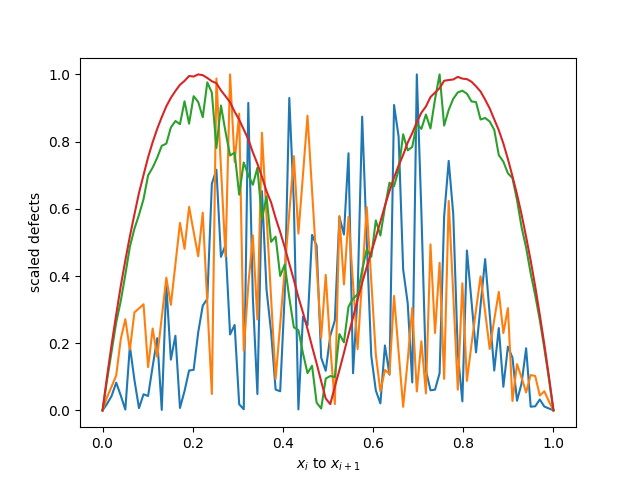
\includegraphics[width=0.7\linewidth]{./figures/rk4_with_hb4_p2_scaled_defects_small_steps}
\caption{Scaled defects small steps taken RK4 with HB4 on problem 2 at an absolute tolerance of $10^{-6}$ mapped onto $[0, 1]$.}
\label{fig:rk4_with_hb4_p2_scaled_defects_small_steps}
\end{figure}

\paragraph{Problem 3 results}
Figures $\ref{fig:rk4_with_hb4_p3_global_defect}$, $\ref{fig:rk4_with_hb4_p3_global_error}$ and $\ref{fig:rk4_with_hb4_p3_scaled_defects}$ shows the results of using RK4 with HB4 on Problem 3. We note that an absolute tolerance of $10^{-6}$ is applied on the maximum defect within the step and this can be shown to occur at $0.2h$ and $0.4h$ along a step of size, h. See Figure $\ref{fig:rk4_with_hb4_p3_scaled_defects}$, to see the scaled defect reaching a maximum near these points. We note that we are able to successfully control the defect of the continuous numerical solution using this approach, see Figure $\ref{fig:rk4_with_hb4_p3_global_defect}$. 

\begin{figure}[H]
\centering
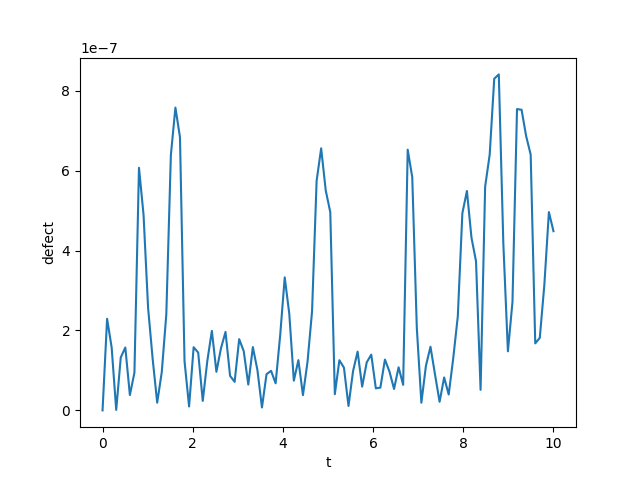
\includegraphics[width=0.7\linewidth]{./figures/rk4_with_hb4_p3_global_defect}
\caption{Defect across the entire domain for RK4 with HB4 on problem 3 at an absolute tolerance of $10^{-6}$.}
\label{fig:rk4_with_hb4_p3_global_defect}
\end{figure}

\begin{figure}[H]
\centering
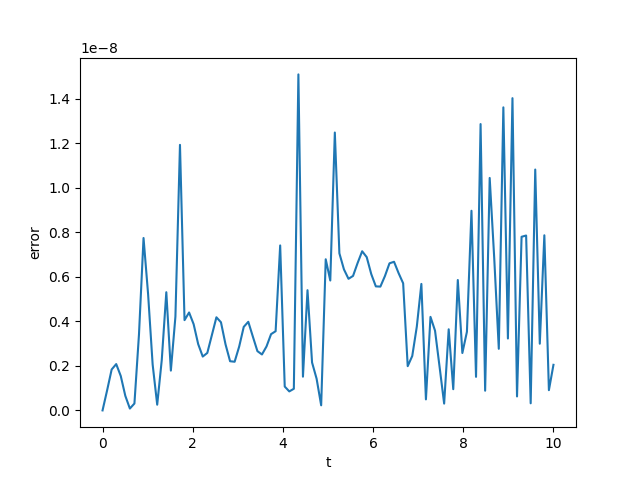
\includegraphics[width=0.7\linewidth]{./figures/rk4_with_hb4_p3_global_error}
\caption{Global Error of RK4 with HB4 for problem 3 at an absolute tolerance of $10^{-6}$.}
\label{fig:rk4_with_hb4_p3_global_error}
\end{figure}

\begin{figure}[H]
\centering
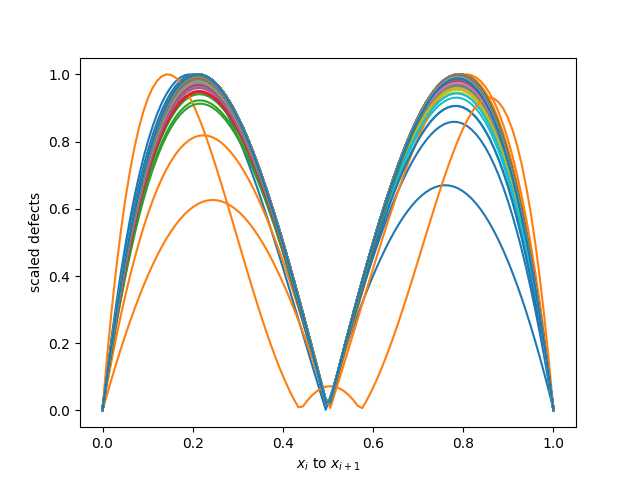
\includegraphics[width=0.7\linewidth]{./figures/rk4_with_hb4_p3_scaled_defects}
\caption{Scaled defects over all steps taken for RK4 with HB4 on problem 3 at an absolute tolerance of $10^{-6}$ mapped onto $[0, 1]$. The shape of the defect stays relatively similar but there are two peaks, one at $0.2h$ and another at $0.8h$.}
\label{fig:rk4_with_hb4_p3_scaled_defects}
\end{figure}

\paragraph{Efficiency data and discussion of the interpolation error}
We now present the number of steps that were taken by the solver to solve each problem along with the number of successful steps.

\begin{table}[h]
\caption {Number of steps taken by RK4 using defect control with HB4.} \label{tab:rk4_with_hb4_nsteps}
\begin{center}
\begin{tabular}{ c c c } 
Problem & successful steps & total steps \\ 
1       & 88                         & 88 \\ 
2       & 59                         & 62 \\
3       & 225                        & 232 \\
\end{tabular}
\end{center}
\end{table}

The Hermite cubic, HB4, is an interpolant of $4^{th}$ order. However, to perform defect control we need to calculate the derivative of this interpolant. Since we are differentiating the interpolant, the order of the derivative is 3. The numerical solution is of order 4 as we are using RK4 and thus the derivative of the interpolant is less accurate than the ODE solution. We need a way to get an interpolant whose derivative is at least of order 4 so that the error of the derivative of the interpolant is not larger than the error of the discrete numerical solution obtained from the RK4 method.

To do that, in the next section, we will introduce a new interpolation scheme based on a Hermite-Birkhoff interpolant which is of $6^{th}$ order and will thus have a derivative of order 5.

\subsection{RK4 with a $6^{th}$ order Hermite-Birkhoff interpolant}
We first start by noting that this interpolant is a multistep interpolant as it depends on the previous step.

Suppose that the step taken by a solver to go from $t_i$ to $t_{i + 1}$ is of size $h$. We can define the size of the step from $t_{i - 1}$ to $t_i$ by using a weight $\alpha$ such that the size of the step from $t_{i - 1}$ to $t_i$ is $\alpha$h. Then given the solution values and the derivative values at all the three points, i.e, $(t_{i-1}, y_{i - 1}, f_{i - 1})$, $(t_i, y_i, f_i)$ and $(t_{i + 1}, y_{i + 1}, f_{i + 1})$, we can fit a two-step quintic interpolant of order 6 defined as such:
\begin{equation}
\begin{split}
u(t_i + \theta h) = d_{0}(\theta) y_{i-1} +  h_id_{1}(\theta)f_{i-1} \\
+ d_{2}(\theta)y_i     +  h_id_{3}(\theta)f_i
+ d_{4}(\theta)y_{i + 1} + h_id_{5}(\theta)f_{i + 1}, \\
\end{split}
\end{equation}
and its derivative is
\begin{equation}
\begin{split}
u'(t_i + \theta h) = d_{0}'(\theta)y_{i-1}/h_i +  d_{1}'(\theta)f_{i-1} \\
+ d_{2}'(\theta)y_i/h_i     +  d_{3}'(\theta)f_i
+ d_{4}'(\theta)y_{i + 1}/h_i + d_{5}'(\theta)f_{i + 1}. \\
\end{split}
\end{equation}
As before, $\theta$ is:
\begin{equation}
\theta = (t - t_i) / h_i.
\end{equation}

This time $\theta$ is allowed to vary between -$\alpha$ and 1 such that $t_i + \theta$h is $t_{i - 1}$ when $\theta$ is $-\alpha$, $t_i$ when $\theta$ is 0 and $t_{i + 1}$ when $\theta$ is 1.

Each of $d_0(\theta)$, $d_1(\theta)$, $d_2(\theta)$, $d_3(\theta)$, $d_4(\theta)$, and $d_5(\theta)$ is a quintic of the form $a\theta^5 + b\theta^4 + c\theta^3 + d\theta^2 + e\theta + f$ where the six coefficients for each can be found by solving a linear system of 6 equations in terms of $\alpha$. The six equations are obtained as follows. First, for $\theta = -\alpha$, only $d_0(\theta)$ evaluates to 1 and all the other quintic polynomials evaluate to 0 as $u(t_i - \alpha h) = u(t_{i - 1}) = y_{i - 1}$. Also at this $\theta$, only the derivative of $d_1(\theta)$ evaluates to 1 and all the other quintic polynomials' derivatives evaluate to 0 as $u'(t_i - \alpha h) = u'(t_{i - 1}) = f_{i - 1}$. When $\theta$ is 0, only $d_2(\theta)$ evaluates to 1 and all the other polynomials evaluate to 0 as $u(t_i - 0(h)) = u(t_i) = y_i$. Also at this $\theta$ value, only the derivative of $d_3(\theta)$ evaluates to 1 and all the other quintic polynomial derivatives evaluate to 0 as $u'(t_i - 0(h)) = u'(t_i) = f_i$. When $\theta$ is 1, only $d_4(\theta)$ evaluates to 1 and all the other polynomials evaluate to 0 as $u(t_i + 1(h)) = u(t_{i+1}) = y_{i+1}$. Also at this $\theta$, only the derivative of $d_5(\theta)$ evaluates to 1 and all the other quintic polynomial derivatives evaluate to 0 as $u'(t_i - 1(h)) = u'(t_{i+1}) = f_{i+1}$. With these six conditions, we can get six equations for each quintic in terms of $\alpha$ and, using a symbolic management package, we can solve all of these to find the six quintic polynomials. (Their coefficients will be given in terms of $\alpha$.)

We again note that as the solver is stepping across the problem domain, these interpolants are constructed for no additional cost in terms of evaluation of $f(t, y(t))$. We just need to store $(t_{i-1}, y_{i - 1}, f_{i - 1})$, $(t_i, y_i, f_i)$ and $(t_{i + 1}, y_{i + 1}, f_{i + 1})$ as these quantities are being computed by the RK method. We will also observe that the defect peaks at two positions within the new step, $[t_i, t_{i+1}]$, and thus, we can find the maximum defect by only sampling the defect twice. This technique provides an efficient defect control of a continuous approximate solution.

The interpolant defined as above will be referred to as `HB6' for the remainder of this chapter. We note that it is of order 6 and its derivative is of order 5.

We now note that for RK4 as the solution values are only accurate to $4^{th}$ order. We want the derivative of the interpolant to be of order 4 or higher so that interpolation error is relatively negligible. This scheme satisfies this condition and we will see below how this allows us to take fewer time steps to solve a given problem than when HB4 was used with RK4.

\paragraph{Problem 1 results}
Figures $\ref{fig:rk4_with_hb6_p1_global_defect}$, $\ref{fig:rk4_with_hb6_p1_global_error}$ and $\ref{fig:rk4_with_hb6_p1_scaled_defects}$ shows the results of using RK4 with HB6 on Problem 1. We note that an absolute tolerance of $10^{-6}$ is applied on the maximum defect within the step and this can be shown to occur at $0.3h$ and $0.8h$ along a step of size, h. See Figure $\ref{fig:rk4_with_hb6_p1_scaled_defects}$, to see the scaled defect reaching a maximum near these points. We note that we are able to successfully control the defect of the continuous numerical solution using this approach; see Figure $\ref{fig:rk4_with_hb6_p1_global_defect}$. 

\begin{figure}[H]
\centering
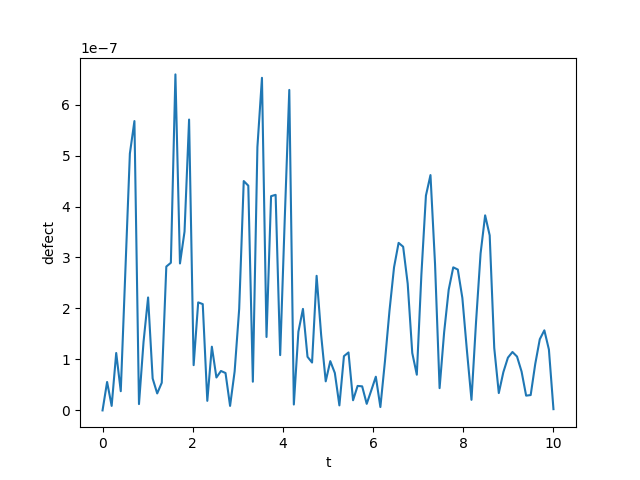
\includegraphics[width=0.7\linewidth]{./figures/rk4_with_hb6_p1_global_defect}
\caption{Defect across the entire domain for RK4 with HB6 on problem 1 at an absolute tolerance of $10^{-6}$.}
\label{fig:rk4_with_hb6_p1_global_defect}
\end{figure}

\begin{figure}[H]
\centering
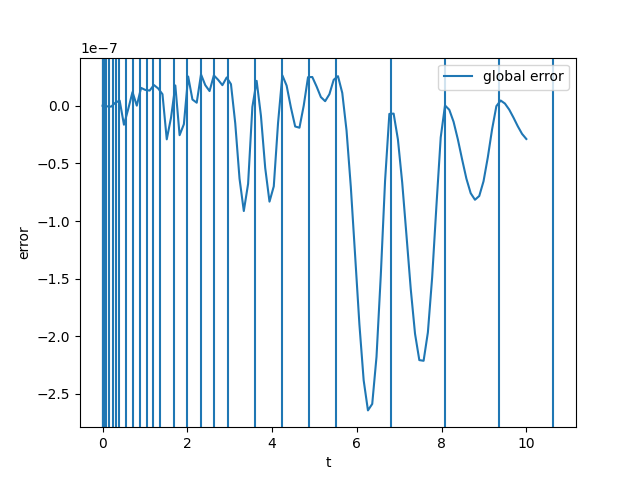
\includegraphics[width=0.7\linewidth]{./figures/rk4_with_hb6_p1_global_error}
\caption{Global Error for RK4 with HB6 on problem 1 at an absolute tolerance of $10^{-6}$.}
\label{fig:rk4_with_hb6_p1_global_error}
\end{figure}

\begin{figure}[H]
\centering
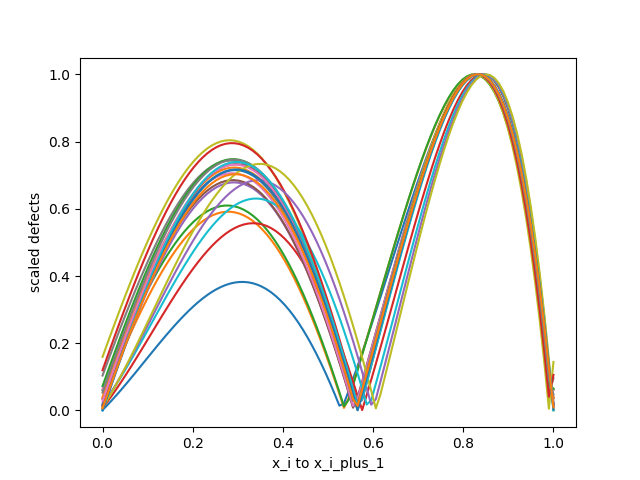
\includegraphics[width=0.7\linewidth]{./figures/rk4_with_hb6_p1_scaled_defects}
\caption{Scaled defects for RK4 with HB6 on problem 1 at an absolute tolerance of $10^{-6}$ mapped into $[0, 1]$.}
\label{fig:rk4_with_hb6_p1_scaled_defects}
\end{figure}

\paragraph{Problem 2 results}
Figures $\ref{fig:rk4_with_hb6_p2_global_defect}$, $\ref{fig:rk4_with_hb6_p2_global_error}$ and $\ref{fig:rk4_with_hb6_p2_scaled_defects}$ shows the results of using the modification of RK4 with HB6 on Problem 2. We note that an absolute tolerance of $10^{-6}$ is applied on the maximum defect within the step and this can be shown to occur at $0.8h$ along a step of size, h. See Figure $\ref{fig:rk4_with_hb6_p2_scaled_defects}$, to see the scaled defect reaching a maximum near these points. We note that we are able to successfully control the defect of the continuous numerical solution using this approach, see Figure $\ref{fig:rk4_with_hb6_p2_global_defect}$. For Problem 2, the defect is noisy on small steps and we do not get two clean peaks. However, we note that we quite consistently get the maximum defects at $0.4h$ and $0.8h$ and thus we only require two samplings.

\begin{figure}[H]
\centering
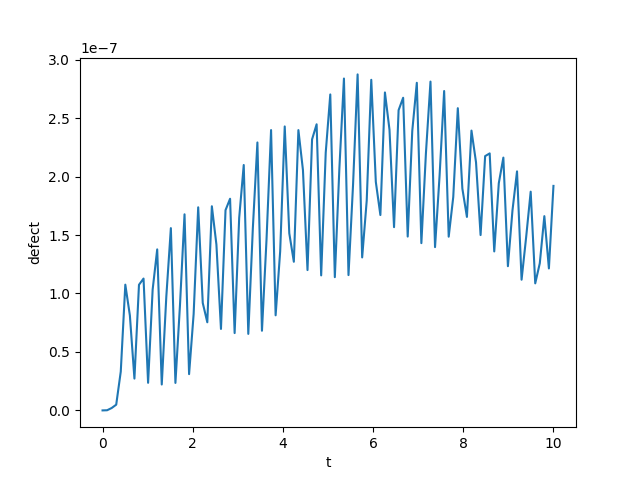
\includegraphics[width=0.7\linewidth]{./figures/rk4_with_hb6_p2_global_defect}
\caption{Defect across the entire domain for RK4 with HB6 on problem 2 at an absolute tolerance of $10^{-6}$.}
\label{fig:rk4_with_hb6_p2_global_defect}
\end{figure}

\begin{figure}[H]
\centering
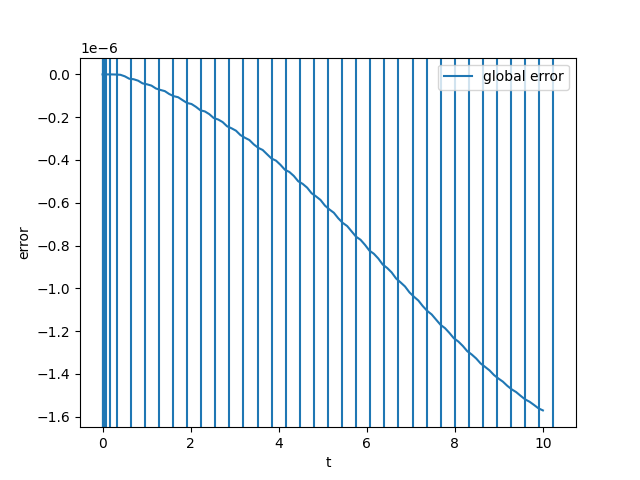
\includegraphics[width=0.7\linewidth]{./figures/rk4_with_hb6_p2_global_error}
\caption{Global Error for RK4 with HB6 on problem 2 at an absolute tolerance of $10^{-6}$.}
\label{fig:rk4_with_hb6_p2_global_error}
\end{figure}

\begin{figure}[H]
\centering
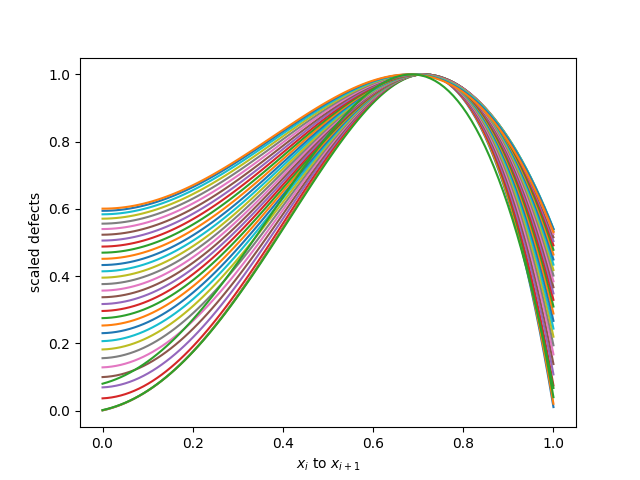
\includegraphics[width=0.7\linewidth]{./figures/rk4_with_hb6_p2_scaled_defects}
\caption{Scaled defects for RK4 with HB6 on problem 2 at an absolute tolerance of $10^{-6}$ mapped into $[0, 1]$.}
\label{fig:rk4_with_hb6_p2_scaled_defects}
\end{figure}

\begin{figure}[H]
\centering
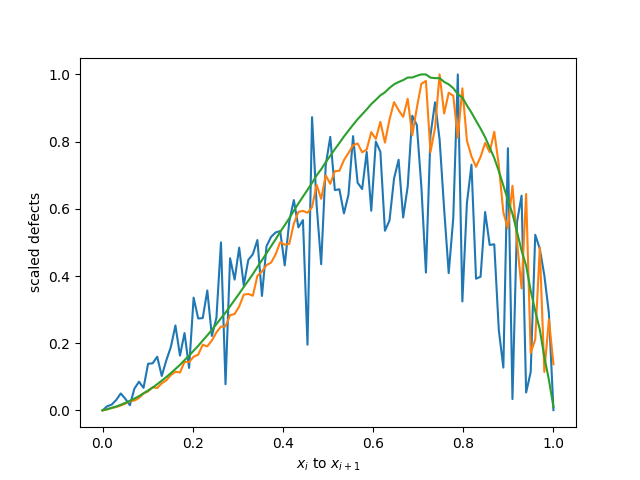
\includegraphics[width=0.7\linewidth]{./figures/rk4_with_hb6_p2_scaled_defects_small_steps}
\caption{Scaled defects for RK4 with HB6 on small steps on problem 2 at an absolute tolerance of $10^{-6}$ mapped into $[0, 1]$. Despite the noise, the maximum defect occurs near $0.8h$.}
\label{fig:rk4_with_hb6_p2_scaled_defects_small_steps}
\end{figure}

\paragraph{Problem 3 results}
Figures $\ref{fig:rk4_with_hb6_p3_global_defect}$, $\ref{fig:rk4_with_hb6_p3_global_error}$ and $\ref{fig:rk4_with_hb6_p3_scaled_defects}$ shows the results of using RK4 with HB6 on Problem 3. We note that an absolute tolerance of $10^{-6}$ is applied on the maximum defect within the step and this can be shown to occur at $0.8h$ along a step of size, h. See Figure $\ref{fig:rk4_with_hb6_p3_scaled_defects}$, to see the scaled defect reaching a maximum near these points. We note that we are able to successfully control the defect of the continuous numerical solution using this approach, see Figure $\ref{fig:rk4_with_hb6_p3_global_defect}$. 


\begin{figure}[H]
\centering
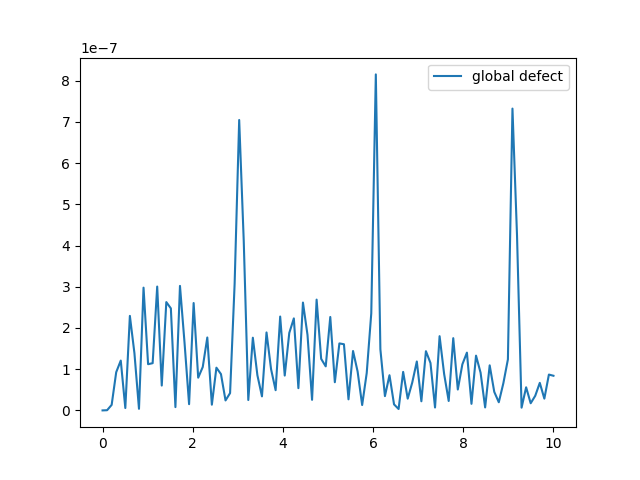
\includegraphics[width=0.7\linewidth]{./figures/rk4_with_hb6_p3_global_defect}
\caption{Defect across the entire domain for RK4 with HB6 on problem 3 at an absolute tolerance of $10^{-6}$.}
\label{fig:rk4_with_hb6_p3_global_defect}
\end{figure}

\begin{figure}[H]
\centering
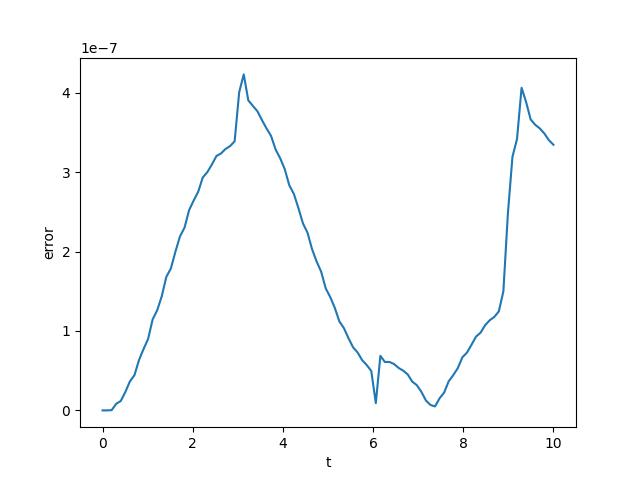
\includegraphics[width=0.7\linewidth]{./figures/rk4_with_hb6_p3_global_error}
\caption{Global Error for RK4 with HB6 on problem 3 at an absolute tolerance of $10^{-6}$.}
\label{fig:rk4_with_hb6_p3_global_error}
\end{figure}

\begin{figure}[H]
\centering
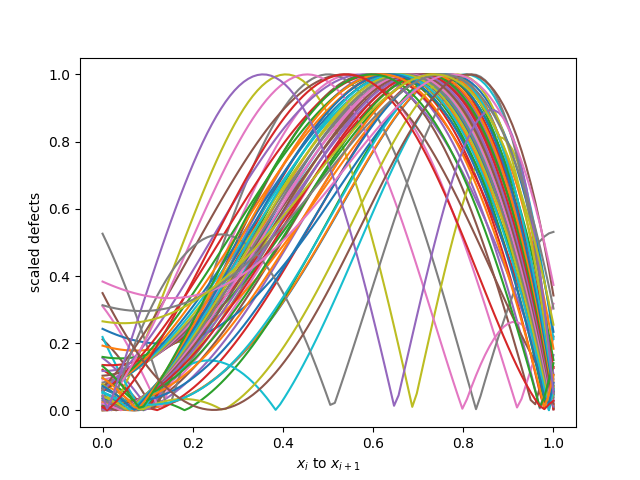
\includegraphics[width=0.7\linewidth]{./figures/rk4_with_hb6_p3_scaled_defects}
\caption{Scaled defects for RK4 with HB6 on problem 3 at an absolute tolerance of $10^{-6}$ mapped into $[0, 1]$.}
\label{fig:rk4_with_hb6_p3_scaled_defects}
\end{figure}

We note that the defects are not as clean they were in the case with HB4. There are two peaks most of the time at around $0.4h$ and $0.8h$ but as was the case in the third problem, the peak sometimes appears at $0.6h$. However, we can see that the defect is still being controlled. We will also see that it is twice as fast as it uses around half the number of steps as HB4.

\begin{table}[h]
\caption {Number of steps taken by RK4 when modified to do defect control with HB6 vs HB4.} \label{tab:rk4_with_hb6_nsteps}
\begin{center}
\begin{tabular}{ c c c c c } 
Problem & succ. steps HB4 & succ. steps HB6 & nsteps HB4  & nsteps HB6 \\ 
1       & 88                 &        27          & 88         & 27 \\ 
2       & 59                 &        36          & 62         & 40 \\
3       & 225                &        62          & 232        & 73 \\
\end{tabular}
\end{center}
\end{table}

Table $\ref{tab:rk4_with_hb6_nsteps}$ shows how the number of steps is less than half when we use HB6 as opposed to HB4. This is entirely because the error of the interpolant and its derivative are smaller than the error of the discrete solution values at the end of each step.

\paragraph{Issues with $\alpha$ values}
The issue with this scheme is that the interpolant is a multistep interpolant while the Runge-Kutta method is a one step method. The Hermite Birkhoff interpolant, HB6, is based on two steps and the parameter $\alpha$ defines how big the previous step is compared to the actual step. The error term in the Hermite-Birkhoff interpolant is minimised when the size of the two steps are the same size, i.e, when $\alpha$ is 1. The error term is proportional to $(t + \alpha)^2t^2(t - 1)^2$. When $\alpha$ differs from 1, the accuracy of the interpolant is reduced.

In Figure $\ref{fig:hb6_alpha_v_shape}$, we show the results of a simple experiment to illustrate how the accuracy of this scheme depends on the value of $\alpha$. We place 3 data points along the t-axis such that their distances apart are $\alpha$h and h for several values of $\alpha$ and we vary h from 1 to $10^{-7}$; we then report on the maximum defect for each h.

\begin{figure}[H]
\centering
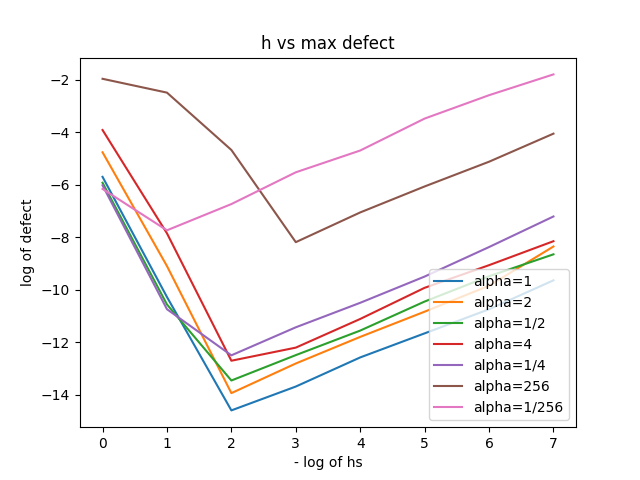
\includegraphics[width=0.7\linewidth]{./figures/hb6_alpha_v_shape}
\caption{HB6 maximum defect based on different values of $\alpha$.}
\label{fig:hb6_alpha_v_shape}
\end{figure}

Figure $\ref{fig:hb6_alpha_v_shape}$ shows that at $\alpha$ = 2, $\frac{1}{2}$, 4 and $\frac{1}{4}$, the defect are comparable to those that we get when $\alpha$ is at 1. However, we see that $\alpha = 256$ and $\frac{1}{256}$, the smallest defect that we can obtain for any $h$ value is much larger.

We note that in solving the 3 test problems, $\alpha$ is very rarely bigger than 4 or smaller than $\frac{1}{4}$ and thus, we can be satisfied with the approach that we have considered in this section. We discuss the situation further in Section $\ref{section:keeping_alpha_at_1}$. We note that in order for the results given in Figure $\ref{fig:hb6_alpha_v_shape}$ to be relevant, we would have to be considering a very sharp tolerance since for reasonable values of $\alpha$, e.g, $2$, $\frac{1}{2}$, $4$ and $\frac{1}{4}$, the interpolants all deliver very small defects of $10^{-12}$ to $10^{-14}$.

Another idea would be to use an even higher order interpolant so as to reduce the interpolation error more. We note that with with the approach we consider here, there is no additional cost to get the higher order interpolant. In the next section, we discuss an $8^{th}$ order interpolant and show how to derive such an interpolant.

\subsection{RK4 with an $8^{th}$ order Hermite-Birkhoff interpolant}
\label{section:HB8_derivation}
\paragraph{Derivation of HB8}
In this section, we discuss a derivation of an $8^{th}$ order interpolant. To derive an 8 order interpolant, we need 4 data points over 3 steps. We need the data values to be $(t_i, y_i, f_i)$, as well as the two previous steps $(t_{i-1}, y_{i-1}, f_{i-1})$ and $(t_{i-2}, y_{i-2}, f_{i-2})$, and the right hand end of the current step step, $(t_{i+1}, y_{i+1}, f_{i+1})$. We present two schemes: 
\begin{itemize}
\item The first scheme has the parameters $\alpha$ and $\beta$ are associated with the previous two steps, so the three steps are of the size $\beta h$, $\alpha h$ and $h$ respectively. Thus the scheme establishes the base step-size to be that of the third step. 

\item The second scheme has the parameter $\alpha$ associated with the rightmost step and the parameter $\beta$ associated with the previous step; the middle step is the base step. Thus the sizes for the steps are $\alpha h$, $h$ and $\beta h$. 

\end{itemize}


\paragraph{First HB8 Scheme}
In the first scheme, the step sizes are $\beta h$, $\alpha h$ and $h$ respectively. The interpolant defined on $(t_{i-2}, y_{i-2}, f_{i-2})$, $(t_{i-1}, y_{i-1}, f_{i-1})$, $(t_i, y_i, f_i)$ and $(t_{i + 1}, y_{i + 1}, f_{i + 1})$ is defined as such:

\begin{equation}
\begin{split}
u(t_i + \theta h) = d_{0}(\theta)y_{i-2} +  h_id_{1}(\theta)f_{i-2} 
+ d_{2}(\theta)y_{i-1}     +  h_id_{3}(\theta)f_{i-1} \\
+ d_{4}(\theta)y_i     +  h_id_{5}(\theta)f_i 
+ d_{6}(\theta)y_{i + 1} + h_id_{7}(\theta)f_{i + 1}, \\
\end{split}
\end{equation}
and the derivative is:
\begin{equation}
\begin{split}
u'(t_i + \theta h) = d_{0}'(\theta)y_{i-2}/h_i +  d_{1}'(\theta)f_{i-2} 
+ d_{2}'(\theta)y_{i-1}/h_i   +  d_{3}'(\theta)f_{i-1} \\
+ d_{4}'(\theta)y_i/h_i       +  d_{5}'(\theta)f_i 
+ d_{6}'(\theta)y_{i + 1}/h_i +  d_{7}'(\theta)f_{i + 1}. \\
\end{split}
\end{equation}
Again $\theta$ is:
\begin{equation}
\theta = (t - t_i) / h_i.
\end{equation}

This time $\theta$ is allowed to vary between $-\alpha-\beta$ and 1 such that $t_i + \theta$h is $t_{i-2}$ when $\theta$ is $-\alpha-\beta$, $t_{i-1}$ when $\theta$ is $-\alpha$, $t_i$ when $\theta$ is 0 and $t_{i + 1}$ when $\theta$ is 1. Also $d_0(\theta)$, $d_1(\theta)$, $d_2(\theta)$, $d_3(\theta)$, $d_4(\theta)$, $d_5(\theta)$, $d_6(\theta)$ and $d_7(\theta)$ are all septic polynomials that will each have 8 coefficients.

Each septic polynomial is assumed to have the form $a\theta^7 + b\theta^6 + c\theta^5 + d\theta^4 + e\theta^3 + f\theta^2 + g\theta + h$ where the eight coefficients for each can be found in terms of $\alpha$ and $\beta$ by solving a linear system of 8 equations in terms of $\alpha$ and $\beta$. First at $\theta = -\alpha-\beta$, only $d_0(\theta)$ evaluates to 1 and all the other septic polynomials evaluate to 0 as $u(t_i - (\alpha+\beta) h) = u(t_{i - 2}) = y_{i - 2}$. Also at this $\theta$ value, only the derivative of $d_1(\theta)$ evaluates to 1 and all the other septic polynomial derivatives evaluate to 0 as $u'(t_i - (\alpha+\beta) h) = u'(t_{i - 2}) = f_{i - 2}$. When $\theta = -\alpha$, only $d_2(\theta)$ evaluates to 1 and all the other septic polynomials evaluate to 0 as $u(t_i - \alpha h) = u(t_{i - 1}) = y_{i - 1}$. Also at this $\theta$ value, only the derivative of $d_3(\theta)$ evaluates to 1 and all the other septic polynomial derivatives evaluate to 0 as $u'(t_i - \alpha h) = u'(t_{i - 1}) = f_{i - 1}$. When $\theta$ is 0, only $d_4(\theta)$ evaluates to 1 and all the other polynomials evaluate to 0 as $u(t_i - 0(h)) = u(t_i) = y_i$. Also at this $\theta$ value, only the derivative of $d_5(\theta)$ evaluates to 1 and all the other septic polynomial derivatives evaluate to 0 as $u'(t_i - 0(h)) = u'(t_i) = f_i$. When $\theta$ is 1, only $d_6(\theta)$ evaluates to 1 and all the other polynomials evaluate to 0 as $u(t_i + 1(h)) = u(t_{i+1}) = y_{i+1}$. Also at this $\theta$ value, only the derivative of $d_7(\theta)$ evaluates to 1 and all the other septic polynomial derivatives evaluate to 0 as $u'(t_i - 1(h)) = u'(t_{i+1}) = f_{i+1}$. With these eight conditions, we can get eight equations for each polynomial in terms of $\alpha$ and $\beta$ and, using a symbolic management package, we can solve all of these to find the eight septic polynomials.

We again note that as the solver is stepping through the problem, these interpolants can be obtained without the need for any extra evaluations of $f$. We just need to store the 4 data points $(t_{i-1}, y_{i - 1}, f_{i - 1})$, $(t_{i-1}, y_{i - 1}, f_{i - 1})$, $(t_i, y_i, f_i)$ and $(t_{i + 1}, y_{i + 1}, f_{i + 1})$.

The interpolant defined as above will be referred to as `HB8 First Scheme' for the remainder of this chapter. We note that it is of order 8 and its derivative is of order 7.

Unfortunately, this scheme has a serious issue. The accuracy of the interpolant is very sensitive to a slight change in $\alpha$ and/or $\beta$. This is because the error term is now proportional to $(t + \alpha + \beta)^2(t+\alpha)^2(t)^2(t-1)^2$. We note that the first term depends on both $\alpha$ and $\beta$ and thus very small deviations of these values from 1 will result in reduced accuracy. 

In Figure $\ref{fig:hb8_first_scheme_alpha_beta_test}$, we present the results of a simple experiment to illustrate this issue. We place 4 data points along the t-axis such that their distances apart are $\beta h$, $\alpha h$ and $h$ for several values of $\alpha$ and $\beta$ and we vary h from 1 to $10^{-10}$; we then report on the order of the maximum defect at each h for these values.

\begin{figure}[H]
\centering
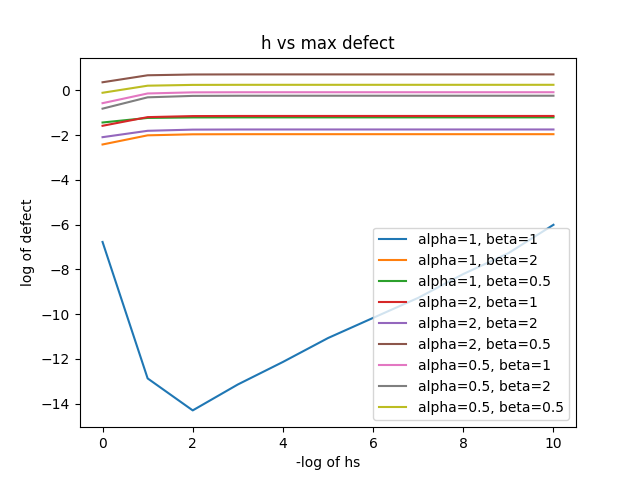
\includegraphics[width=0.7\linewidth]{./figures/hb8_first_scheme_alpha_beta_test}
\caption{HB8 First Scheme - maximum size of the defect based on different values of $\alpha$ and $\beta$.}
\label{fig:hb8_first_scheme_alpha_beta_test}
\end{figure}

From Figure $\ref{fig:hb8_first_scheme_alpha_beta_test}$, we can see the issue with this scheme. It only works if both $\alpha$ and $\beta$ are 1 and even small deviations from 1 for either $\alpha$ or $\beta$ drastically reduces the accuracy. More importantly, we can never halve the step with this method as if either $\alpha$ or $\beta$ is 2, the interpolant is not accurate to even one order of magnitude. We will now consider a second scheme which is more stable with respect to changes in $\alpha$ and $\beta$.

\paragraph{Second HB8 Scheme}
In this second scheme, we still use a 3 step interpolant with 4 data points $(t_{i-1}, y_{i-1}, f_{i-1})$, $(t_{i-2}, y_{i-2}, f_{i-2})$, $(t_{i}, y_{i}, f_{i})$ and $(t_{i+1}, y_{i+1}, f_{i+1})$ but now the distance between the points are $\alpha h$, $h$ and then $\beta h$. The middle step is the base step. This way the error term is approximately proportional to $(t- (1+\alpha))^2(t-1)^2t^2(t+\beta)^2$. We avoid the $(t-(\alpha+\beta))^2$ factor. We will show that this scheme is more resilient to changes in $\alpha$ and $\beta$.

Its derivation is very similar to the first scheme. The equation for the interpolant is:
\begin{equation}
\begin{split}
u(t_i + \theta h) = d_{0}(\theta)y_{i-2} +  h_id_{1}(\theta)f_{i-2} 
+ d_{2}(\theta)y_{i-1}     +  h_id_{3}(\theta)f_{i-1} \\
+ d_{4}(\theta)y_i     +  h_id_{5}(\theta)f_i 
+ d_{6}(\theta)y_{i + 1} + h_id_{7}(\theta)f_{i + 1}, \\
\end{split}
\end{equation}
and its derivative is:
\begin{equation}
\begin{split}
u'(t_i + \theta h) = d_{0}'(\theta)y_{i-2}/h_i +  d_{1}'(\theta)f_{i-2}
+ d_{2}'(\theta)y_{i-1}/h_i   +  d_{3}'(\theta)f_{i-1} \\
+ d_{4}'(\theta)y_i/h_i       +  d_{5}'(\theta)f_i
+ d_{6}'(\theta)y_{i + 1}/h_i +  d_{7}'(\theta)f_{i + 1}. \\
\end{split}
\end{equation}
Again $\theta$ is:
\begin{equation}
\theta = (t - t_i) / h_i.
\end{equation}

This time $\theta$ is allowed to vary between $-1-\alpha$ and $\beta$ such that $t_i + \theta h$ is $t_{i-2}$ when $\theta$ is $-1-\alpha$, $t_{i-1}$ when $\theta$ is -1, $t_i$ when $\theta$ is 0 and $t_{i + 1}$ when $\theta$ is $\beta$. Also $d_0(\theta)$, $d_1(\theta)$, $d_2(\theta)$, $d_3(\theta)$, $d_4(\theta)$, $d_5(\theta)$, $d_6(\theta)$ and $d_7(\theta)$ are all septic polynomials and will each have 8 conditions from which we can build a system to find their coefficients in terms of $\alpha$ and $\beta$.

Each is a septic of the form $a\theta^7 + b\theta^6 + c\theta^5 + d\theta^4 + e\theta^3 + f\theta^2 + g\theta + h$ where the eight coefficients for each can be found in terms of $\alpha$ and $\beta$ by solving a linear system of 8 equations in terms of $\alpha$ and $\beta$. First at $\theta = -1-\alpha$, only $d_0(\theta)$ evaluates to 1 and all the other septic polynomials evaluate to 0 as $u(t_i - (1+\alpha) h) = u(t_{i - 2}) = y_{i - 2}$. Also at this $\theta$ value, only the derivative of $d_1(\theta)$ evaluates to 1 and all the other septic polynomial derivatives evaluate to 0 as $u'(t_i - (1+\alpha) h) = u'(t_{i - 2}) = f_{i - 2}$. When $\theta = -1$, only $d_2(\theta)$ evaluates to 1 and all the other septic polynomials evaluate to 0 as $u(t_i - 1(h)) = u(t_{i - 1}) = y_{i - 1}$. Also at this $\theta$ value, only the derivative of $d_3(\theta)$ evaluates to 1 and all the other septic polynomials' derivatives evaluate to 0 as $u'(t_i - 1(h)) = u'(t_{i - 1}) = f_{i - 1}$. When $\theta$ is 0, only $d_4(\theta)$ evaluates to 1 and all the other polynomials evaluate to 0 as $u(t_i - 0(h)) = u(t_i) = y_i$. Also at this $\theta$ value, only the derivative of $d_5(\theta)$ evaluates to 1 and all the other septic polynomials' derivatives evaluate to 0 as $u'(t_i - 0(h)) = u'(t_i) = f_i$. When $\theta$ is $\beta$, only $d_6(\theta)$ evaluates to 1 and all the other polynomials evaluate to 0 as $u(t_i + \beta h) = u(t_{i+1}) = y_{i+1}$. Also at this $\theta$ value, only the derivative of $d_7(\theta)$ evaluates to 1 and all the other septic polynomial derivatives evaluate to 0 as $u'(t_i - \beta h) = u'(t_{i+1}) = f_{i+1}$. With these eight conditions, we can get eight equations for each septic in terms of $\alpha$ and $\beta$ and using a symbolic management package, we can solve all of these to find the 8 coefficients for each septic polynomial.

We now perform a simple experiment to show that the resultant interpolant is more resilient to changes in $\alpha$ and $\beta$. We place 4 data points along the x-axis such that their distance apart are $\alpha h$, $h$ and $\beta h$ for several values of $\alpha$ and $\beta$ and we vary $h$ from 1 to $10^{-10}$, we then report on the maximum defect at each $h$ for these values.

\begin{figure}[H]
\centering
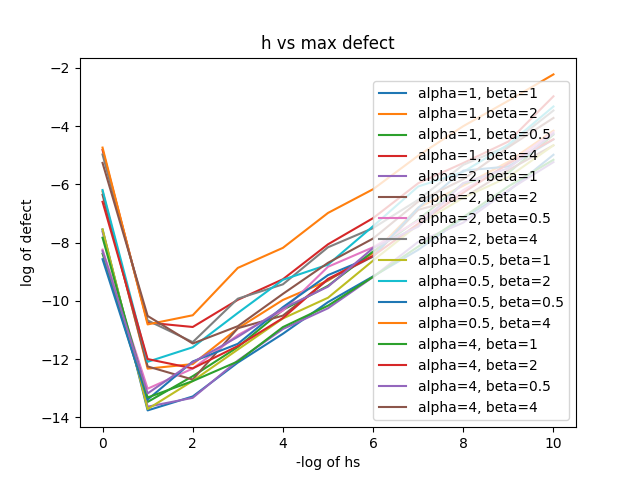
\includegraphics[width=0.7\linewidth]{./figures/hb8_second_scheme_alpha_beta_test}
\caption{HB8 Second Scheme - maximum order of accuracy based on different values of alpha and beta.}
\label{fig:hb8_second_scheme_alpha_beta_test}
\end{figure}

From Figure $\ref{fig:hb8_second_scheme_alpha_beta_test}$, we can see how this scheme is better than the first scheme. We can use $\alpha$ and $\beta$ equal to 2 and to 1/2 and still get a maximum defect of around $10^{-12}$ and we can even be accurate to $10^{-10}$ for both $\alpha$ and $\beta$ equal to 4 and $\frac{1}{4}$. 

For the remainder of this chapter, we will denote this $8^{th}$ order interpolant by HB8. Its derivative has order 7 and any subsequent higher derivative will have one less order.

\paragraph{Results}
We will now use RK4 with the second HB8 scheme and use the new defect control solver to solve the three test problems. We will show that we need to sample the defect only twice to estimate the maximum defect and that this scheme can provide good quality defect control.

\paragraph{Problem 1 results}
Figures $\ref{fig:rk4_with_hb8_p1_global_defect}$, $\ref{fig:rk4_with_hb8_p1_global_error}$ and $\ref{fig:rk4_with_hb8_p1_scaled_defects}$ shows the results of using RK4 with HB8 on Problem 1. We note that an absolute tolerance of $10^{-6}$ is applied on the maximum defect within the step and this can be shown to occur at $0.3h$ and $0.8h$ along a step of size, h. See Figure $\ref{fig:rk4_with_hb8_p1_scaled_defects}$, to see the scaled defect reaching a maximum near these points. We note that we are able to successfully control the defect of the continuous numerical solution using this approach, see Figure $\ref{fig:rk4_with_hb8_p1_global_defect}$. 

\begin{figure}[H]
\centering
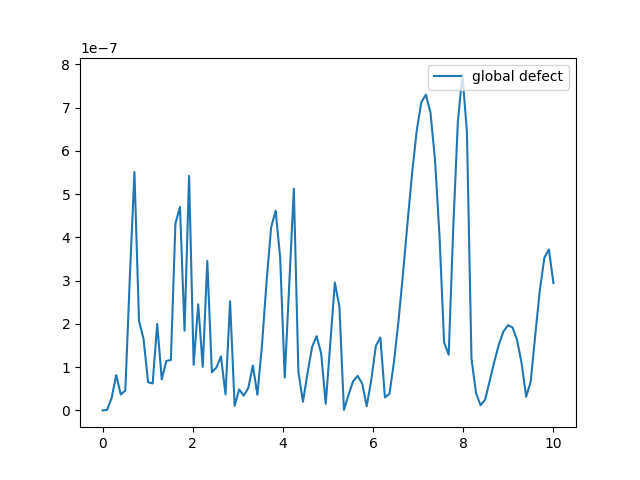
\includegraphics[width=0.7\linewidth]{./figures/rk4_with_hb8_p1_global_defect}
\caption{Defect across the entire domain for RK4 with HB8 on problem 1 at an absolute tolerance of $10^{-6}$.}
\label{fig:rk4_with_hb8_p1_global_defect}
\end{figure}

\begin{figure}[H]
\centering
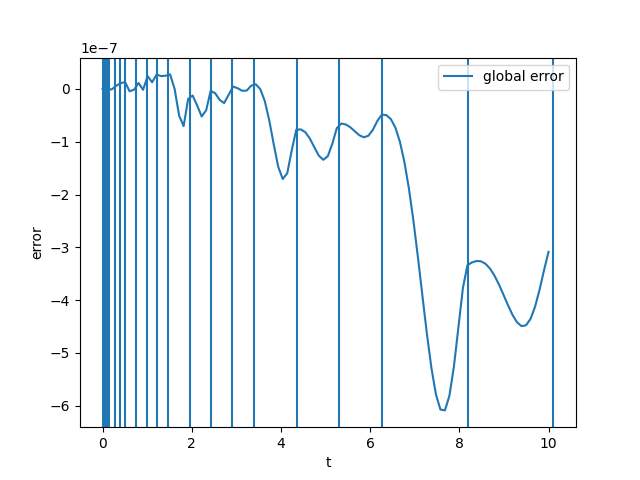
\includegraphics[width=0.7\linewidth]{./figures/rk4_with_hb8_p1_global_error}
\caption{Global Error for RK4 with HB8 on problem 1 at an absolute tolerance of $10^{-6}$.}
\label{fig:rk4_with_hb8_p1_global_error}
\end{figure}

\begin{figure}[H]
\centering
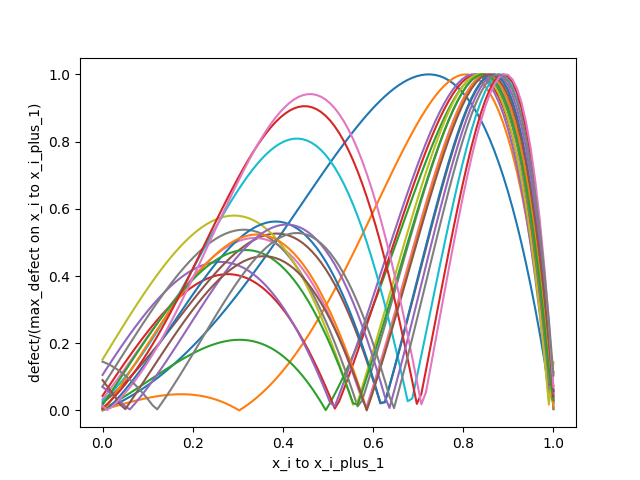
\includegraphics[width=0.7\linewidth]{./figures/rk4_with_hb8_p1_scaled_defects}
\caption{Scaled defects for RK4 with HB8 on problem 1 at an absolute tolerance of $10^{-6}$ mapped into $[0, 1]$.}
\label{fig:rk4_with_hb8_p1_scaled_defects}
\end{figure}

\paragraph{Problem 2 results}
Figures $\ref{fig:rk4_with_hb8_p2_global_defect}$, $\ref{fig:rk4_with_hb8_p2_global_error}$ and $\ref{fig:rk4_with_hb8_p2_scaled_defects}$ shows the results of using RK4 with HB6 on Problem 2. We note that an absolute tolerance of $10^{-6}$ is applied on the maximum defect within the step and this can be shown to occur at $0.8h$ along a step of size, h. See Figure $\ref{fig:rk4_with_hb8_p2_scaled_defects}$, to see the scaled defect reaching a maximum near these points. We note that we are able to successfully control the defect of the continuous numerical solution using this approach, see Figure $\ref{fig:rk4_with_hb8_p2_global_defect}$. 

\begin{figure}[H]
\centering
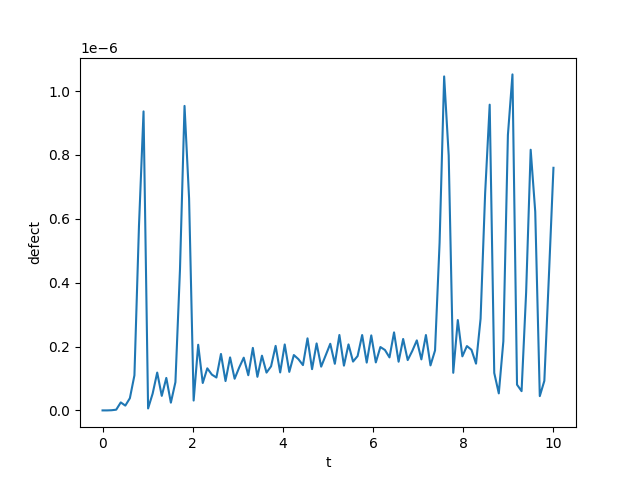
\includegraphics[width=0.7\linewidth]{./figures/rk4_with_hb8_p2_global_defect}
\caption{Defect across the entire domain for RK4 with HB8 on problem 2 at an absolute tolerance of $10^{-6}$.}
\label{fig:rk4_with_hb8_p2_global_defect}
\end{figure}

\begin{figure}[H]
\centering
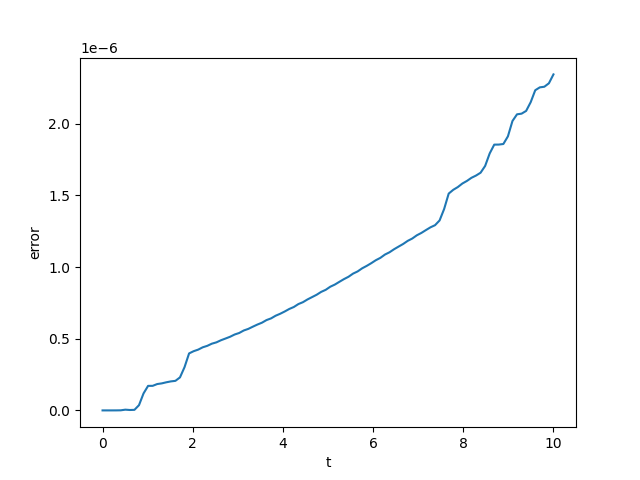
\includegraphics[width=0.7\linewidth]{./figures/rk4_with_hb8_p2_global_error}
\caption{Global Error for RK4 with HB8 on problem 2 at an absolute tolerance of $10^{-6}$.}
\label{fig:rk4_with_hb8_p2_global_error}
\end{figure}

\begin{figure}[H]
\centering
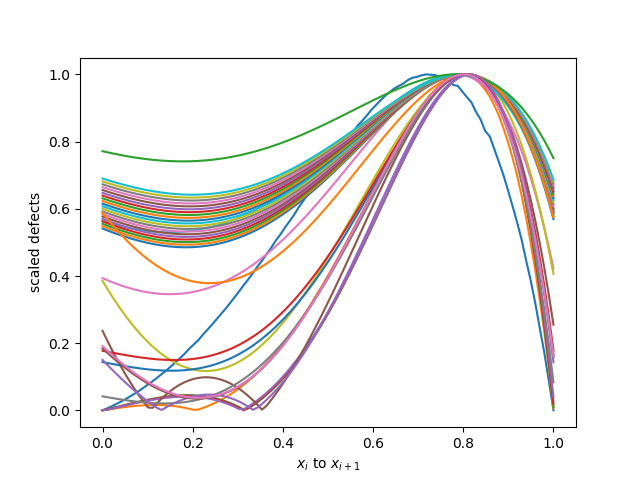
\includegraphics[width=0.7\linewidth]{./figures/rk4_with_hb8_p2_scaled_defects}
\caption{Scaled defects of RK4 with HB8 for problem 2 at an absolute tolerance of $10^{-6}$ mapped into $[0, 1]$.}
\label{fig:rk4_with_hb8_p2_scaled_defects}
\end{figure}

\paragraph{Problem 3 results}
Figures $\ref{fig:rk4_with_hb8_p3_global_defect}$, $\ref{fig:rk4_with_hb8_p3_global_error}$ and $\ref{fig:rk4_with_hb8_p3_scaled_defects}$ shows the results of using RK4 with HB6 on Problem 3. 
We note that an absolute tolerance of $10^{-6}$ is applied on the maximum defect within the step and this can be shown to occur at $0.3h$ or $0.8h$ along a step of size, h.  See Figure $\ref{fig:rk4_with_hb8_p3_scaled_defects}$, to see the scaled defect reaching a maximum near these points. We note that we are able to successfully control the defect of the continuous numerical solution using this approach, see Figure $\ref{fig:rk4_with_hb8_p3_global_defect}$. 

\begin{figure}[H]
\centering
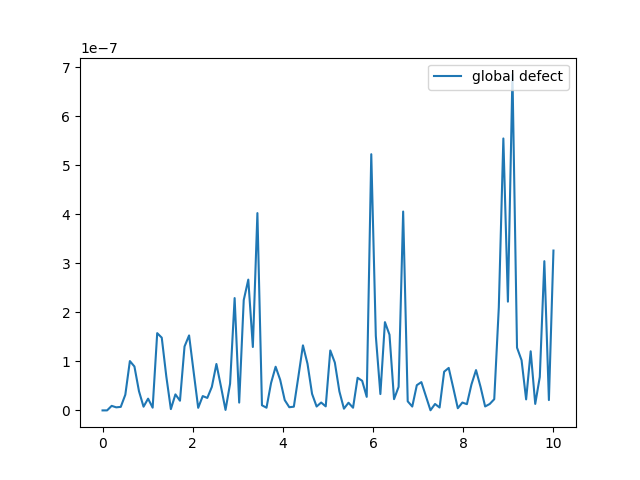
\includegraphics[width=0.7\linewidth]{./figures/rk4_with_hb8_p3_global_defect}
\caption{Defect across the entire domain of RK4 with HB8 on problem 3 at an absolute tolerance of $10^{-6}$.}
\label{fig:rk4_with_hb8_p3_global_defect}
\end{figure}

\begin{figure}[H]
\centering
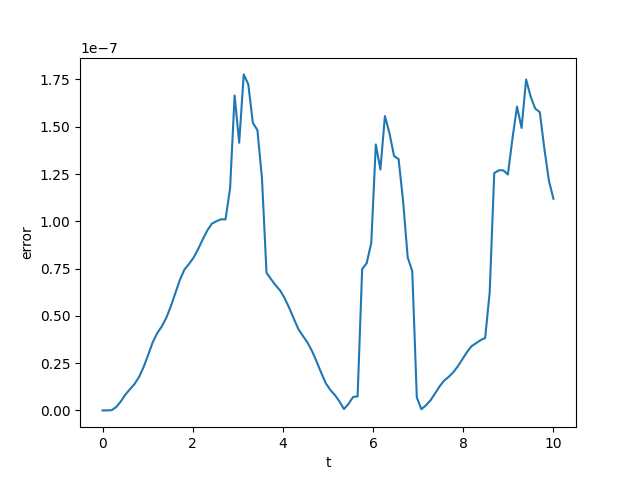
\includegraphics[width=0.7\linewidth]{./figures/rk4_with_hb8_p3_global_error}
\caption{Global Error of RK4 with HB8 on problem 3 at an absolute tolerance of $10^{-6}$.}
\label{fig:rk4_with_hb8_p3_global_error}
\end{figure}

\begin{figure}[H]
\centering
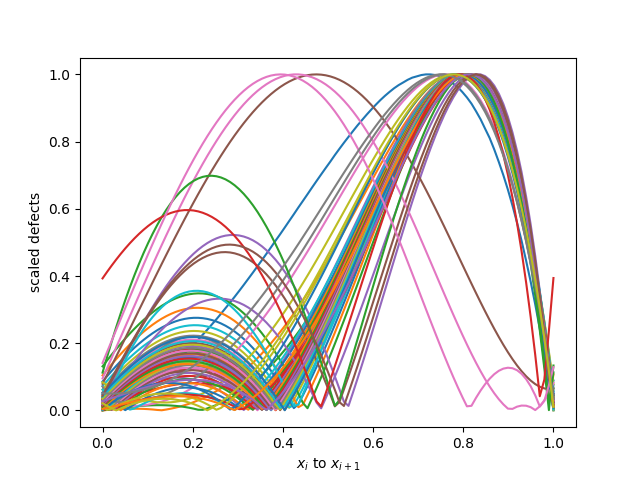
\includegraphics[width=0.7\linewidth]{./figures/rk4_with_hb8_p3_scaled_defects}
\caption{Scaled defects of RK4 with HB8 on problem 3 at an absolute tolerance of $10^{-6}$ mapped onto $[0, 1]$.}
\label{fig:rk4_with_hb8_p3_scaled_defects}
\end{figure}

We note that the defects are not as clean they were in the case with HB4. There are two peaks most of the time at around $0.3h$ and $0.8h$ but as was the case for the third problem in the previous tests, the peak sometimes appears at $0.6h$. However, we can see that the defect is still being controlled and thus that the error is still being controlled. We will also see that it is twice as fast as it uses around half the number of steps as HB4.

\begin{table}[h]
\caption {Number of steps taken by RK4 when modified to do defect control with HB8 vs when modified with HB6.} \label{tab:rk4_with_hb8_nsteps}
\begin{center}
\begin{tabular}{ c c c c c } 
Problem & succ. steps HB8 & succ. steps HB6 & nsteps HB8 & nsteps HB6 \\ 
1       & 20                 &        27          & 20         & 27\\ 
2       & 37                 &        36          & 60         & 40\\
3       & 69                 &        62          & 89         & 73\\
\end{tabular}
\end{center}
\end{table}

From Table $\ref{tab:rk4_with_hb8_nsteps}$, we can see that the number of steps with HB6 and with HB8 are relatively similar. This indicates that the interpolation error is no longer the limiting factor, even in HB6. The limiting factor is the discrete numerical solution which is as required. Thus though we can use RK4 with HB8 at the same cost as modifying RK4 with HB6, using HB8 does not improve the efficiency. Furthermore, HB8 is less stable to changes in $\alpha$ and $\beta$ than HB6 is to changes to $\alpha$. Thus RK4 is best augmented with HB6. However HB8 provides a new opportunity, we can now augment a $6^{th}$ order Runge Kutta method and possibly an $8^{th}$ order Runge-Kutta method, but in the latter case, the interpolation error will still affect the accuracy. Augmenting higher order methods with our HB6 and HB8 schemes is significant because as we have discussed in Section $\ref{section:crk_related_work}$ when using continuous Runge-Kutta solvers to obtain the interpolants, the number of stages grows exponentially with the order of the method. Our scheme is zero-cost and thus effective defect control using this approach will be relatively more efficient.